\subsection{Evaluation Metrics}
Segmentation uses pixel accuracy (non-background), precision, recall, F1, mIoU, and mDice, macro-averaged over the seven LoveDA classes (indices 1--7). Planning uses connectivity before/after planning, proposed-connection count, total/average road length, average nearest-road distance, and path efficiency (straight-line to planned-path ratio; 1 is most direct).

\section{Dataset, Preprocessing, and Experimental Setup}\label{sec:setup}
Data come from LoveDA~\cite{wang2021loveda} (Rural + Urban combined), a benchmark alongside SpaceNet~\cite{vanetten2018} and DeepGlobe~\cite{demir2018}. Images/masks are resized to $560\times560$ (nearest-neighbour for masks), scaled to $[0,1]$ without ImageNet normalisation, with random horizontal/vertical flips and $0^\circ/90^\circ/180^\circ/270^\circ$ rotations at training only. Masks follow the official LoveDA label encoding; index 0 (no-data) is excluded from loss and metrics, and the seven scored classes are Background, Building, Road, Water, Barren, Forest, and Agriculture. The Train split was used for training and the Val split for all reported metrics; epoch selection was also made on validation mIoU, so reported metrics are model-selection-biased and no held-out test set was used. The ten planning tiles (4216--4225) were taken from the unlabelled LoveDA Test/Rural directory, contributing to neither training loss nor epoch selection; carrying no ground-truth masks, their segmentation accuracy is unmeasured, so the planning results describe pipeline behaviour on unseen imagery without a segmentation-accuracy guarantee.

The pipeline is implemented in Python (PyTorch, Hugging Face transformers, OpenCV, scikit-image, NetworkX, SciPy, and Matplotlib) with \texttt{facebook/dinov2-base} as encoder. Training used an NVIDIA RTX A4000 GPU (16 GB); planning ran on an NVIDIA Tesla T4. Table~\ref{tab:train} lists the training configuration. The model trained end-to-end for 10 epochs (encoder at reduced LR), checkpointed on validation-mIoU improvement; epoch 4 (mIoU 0.5380, mDice 0.6891) was selected. Planning was demonstrated on LoveDA image 4216 at the default 5 px connectivity radius, with a separate tile used for the radius-sensitivity experiment.

\begin{table}[t]
\caption{Per-class and overall (macro-averaged) segmentation metrics, epoch-4 model.}\label{tab:seg}
\centering
\begin{tabular}{lrrrr}
\toprule
Class & IoU (\%) & Precision (\%) & Recall (\%) & F1 (\%)\\
\midrule
Background & 54.00 & 62.09 & 80.57 & 70.13\\
Building & 66.77 & 78.77 & 81.43 & 80.08\\
Road & 56.44 & 82.46 & 64.14 & 72.15\\
Water & 71.91 & 84.65 & 82.69 & 83.66\\
Barren & 30.13 & 49.47 & 43.52 & 46.31\\
Forest & 39.86 & 61.51 & 53.11 & 57.00\\
Agriculture & 57.50 & 87.58 & 62.61 & 73.02\\
\midrule
Overall (macro avg.) & 53.80 (mIoU) & 72.36 & 66.87 & 68.91 (mDice)\\
\bottomrule
\end{tabular}
\end{table}

\begin{figure}[t]
\centering
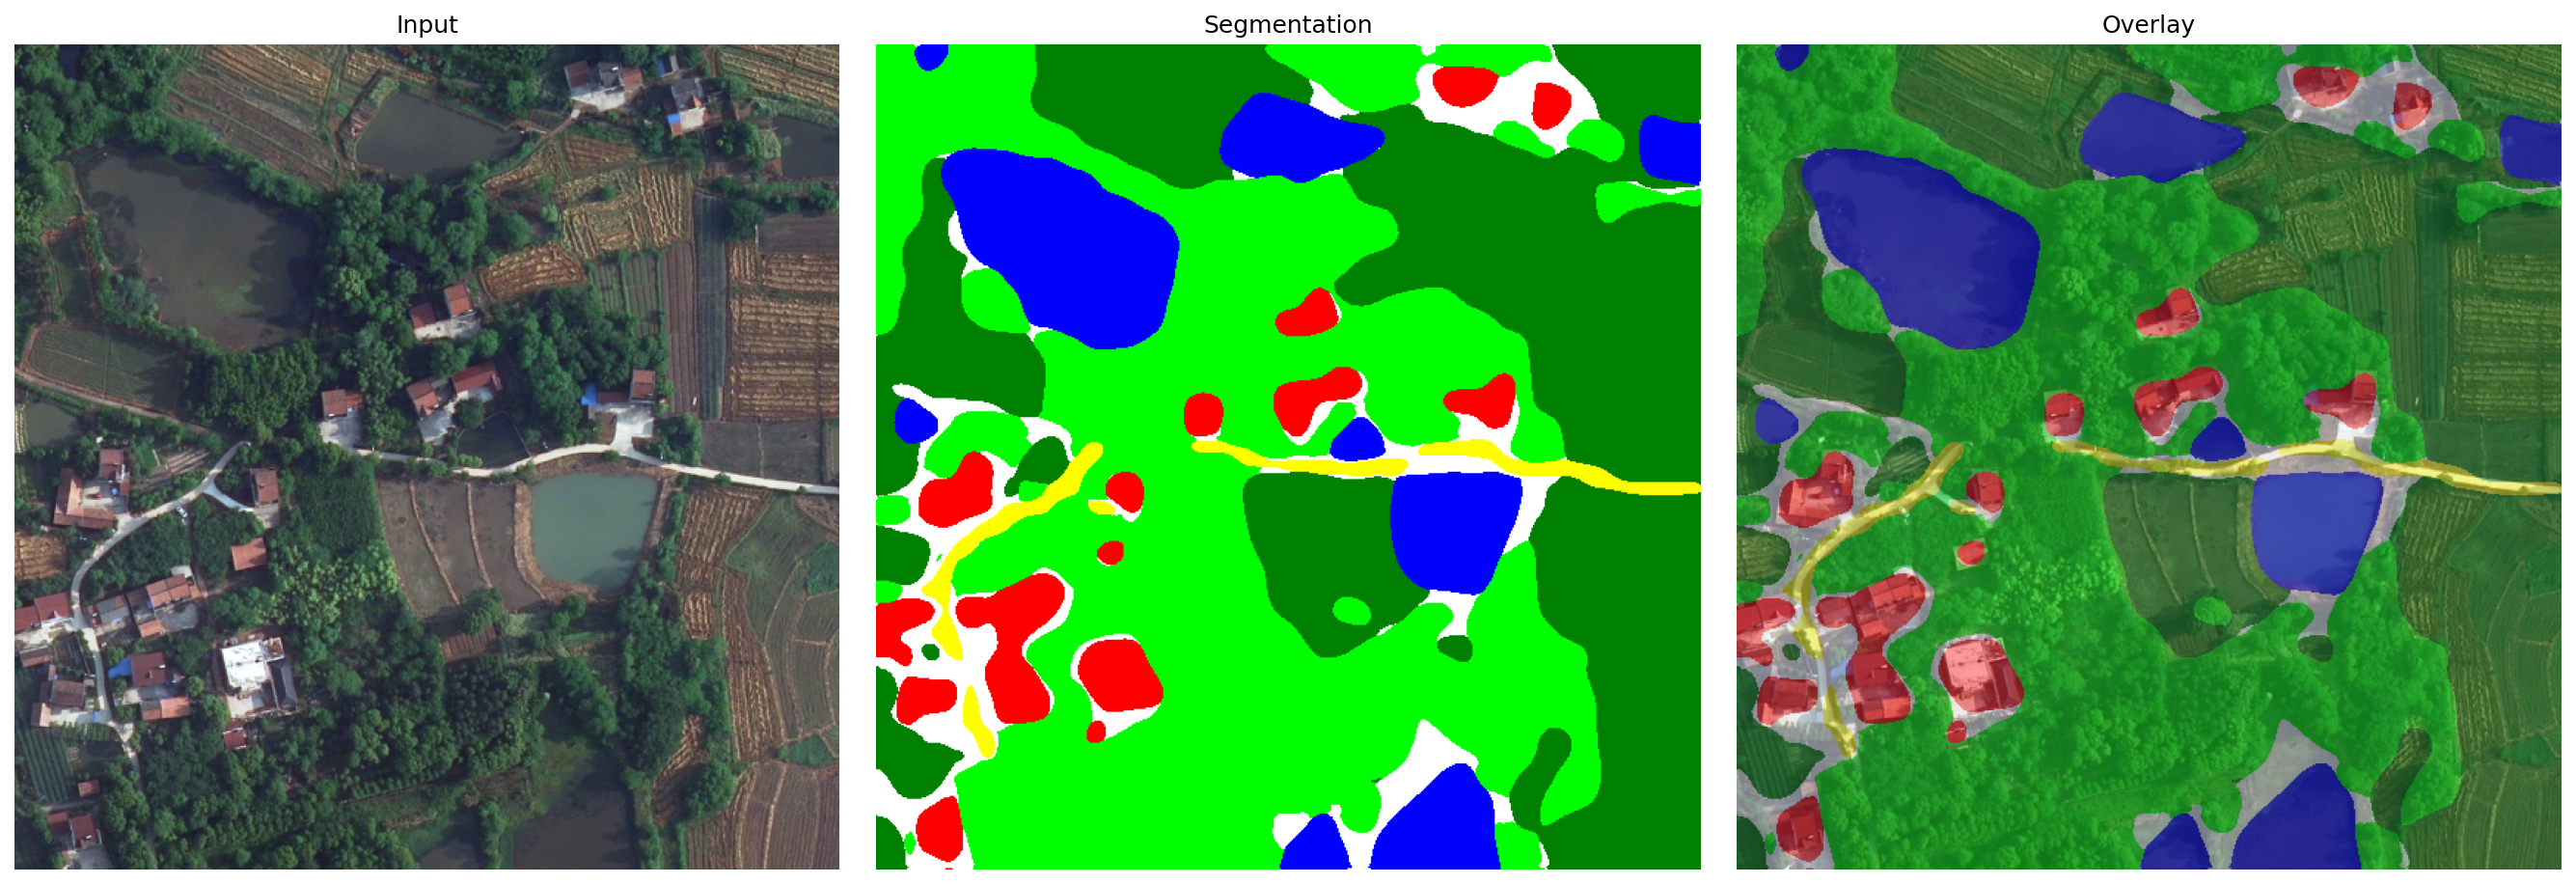
\includegraphics[width=\textwidth]{figs/fig1_segmentation.png}
\caption{Segmentation output for a sample tile. Left: input image. Centre: predicted class map. Right: prediction overlaid on the input.}\label{fig:seg}
\end{figure}

\section{Results and Discussion}
\subsection{Building Detection and Segmentation Results}
On tile 4216, 8-connected component analysis of the Building mask (20-pixel minimum area) yields 14 building instances; at $r=5$ px, 4 connect to the extracted road skeleton and 10 are isolated (Fig.~\ref{fig:plan}, left) -- instance counts, distinct from the pixel-area fractions in Sect.~7.3. Table~\ref{tab:seg} reports per-class and overall metrics of the epoch-4 model (pixel accuracy 71.34\%; Fig.~\ref{fig:seg}). Accuracy peaked at 72.19\% at epoch 2, but epoch 4 was kept since mIoU was the selection criterion. Training loss fell monotonically over 10 epochs (2.0436 to 1.0488); validation mIoU rose from 0.5208 to a peak of 0.5380 at epoch 4 before plateauing (Fig.~\ref{fig:train}), motivating epoch-4 selection despite the continuing loss reduction.

\begin{figure}[t]
\centering
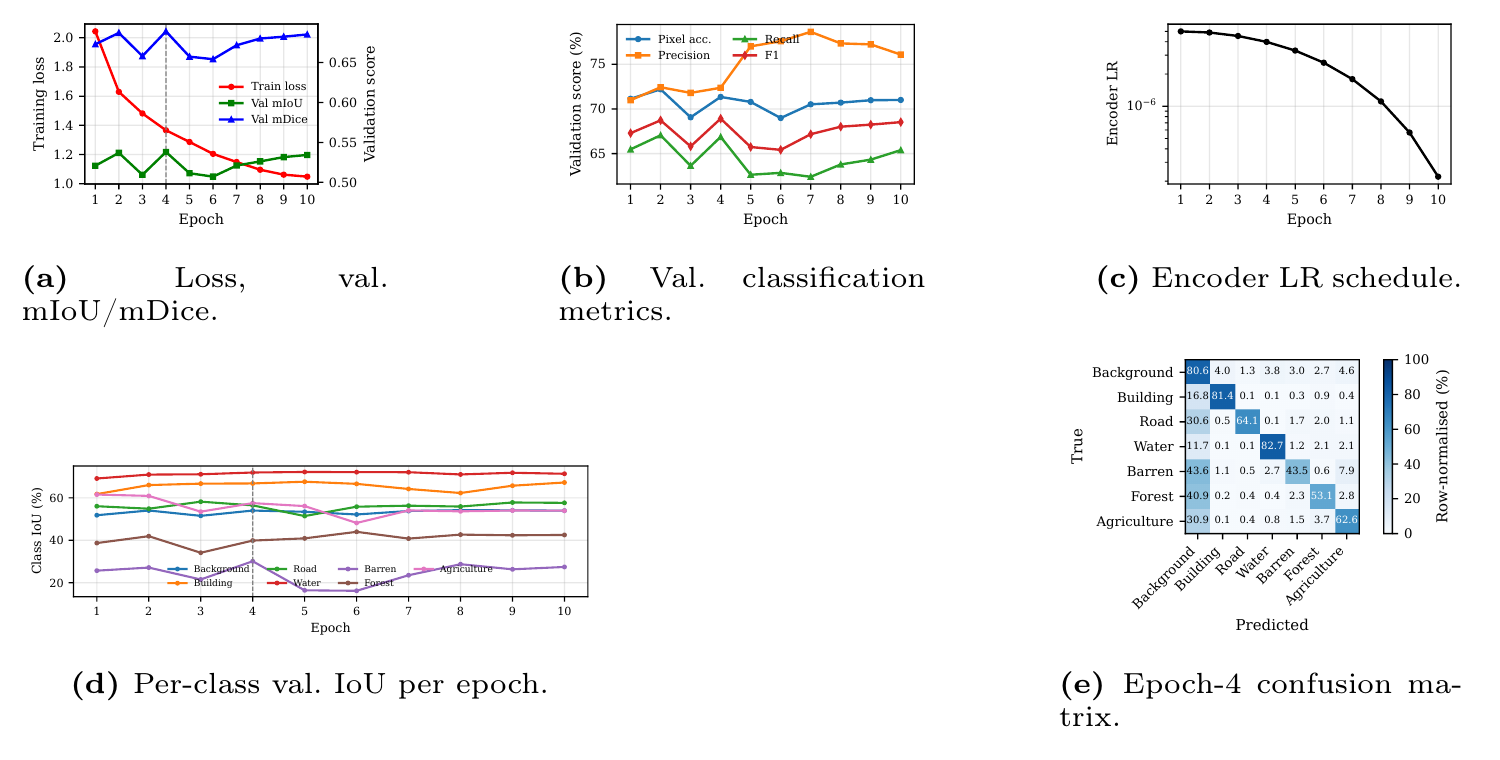
\includegraphics[width=\textwidth]{figs/fig2_training.png}
\caption{Training diagnostics over ten epochs, re-plotted from the training log with official LoveDA class names. Dashed line marks epoch 4 (selected on validation mIoU); all curves are validation-split diagnostics, not held-out test results.}\label{fig:train}
\end{figure}

\subsection{Connectivity, Planning, and Sensitivity Results}
At $r=5$ px, connectivity on the representative tile (14 buildings) rose from 4 (28.57\%) to 14 (100.00\%) via 10 connections totalling 2,029.94 px (mean 202.99 px), mean nearest-road distance 170.78 px, mean path efficiency 0.86 (Fig.~\ref{fig:plan}, right). Table~\ref{tab:tile10} (left) varies $r\in\{3,5,8,10\}$ px on a different tile (15 buildings; 46.67\% connected, 8 connections at $r=5$ px, hence its differing row): a larger radius marks more buildings as already connected, so connections fall from 9 to 6 and length from 1,164.0 to 1,046.1 px, efficiency staying in 0.83--0.86.

\begin{table}[t]
\caption{Left: connectivity-radius sensitivity (separate demonstration tile). Right: aggregate ten-tile planning summary ($r=5$ px).}\label{tab:tile10}
\centering
\begin{minipage}[c]{0.46\textwidth}
\centering
\begin{tabular}{rrrrr}
\toprule
$r$ (px) & Before (\%) & After (\%) & Length (px) & Eff.\\
\midrule
3 & 40.00 & 100.0 & 1164.00 & 0.8605\\
5 & 46.67 & 100.0 & 1130.10 & 0.8502\\
8 & 53.33 & 100.0 & 1074.88 & 0.8529\\
10 & 60.00 & 100.0 & 1046.06 & 0.8307\\
\bottomrule
\end{tabular}
\end{minipage}\hfill
\begin{minipage}[c]{0.50\textwidth}
\centering
\begin{tabular}{lr}
\toprule
Metric & Value\\
\midrule
Images / with proposals & 10 / 8\\
Buildings detected & 54\\
Connected before & 22 (40.74\%)\\
Connected after & 52 (96.30\%)\\
Proposed connections & 30\\
Total proposed length & 4,198.6 px\\
Mean nearest-road dist. & $162.47\pm80.88$ px\\
Mean path efficiency & $0.931\pm0.026$\\
\bottomrule
\end{tabular}
\end{minipage}
\end{table}

\begin{figure}[t]
\centering
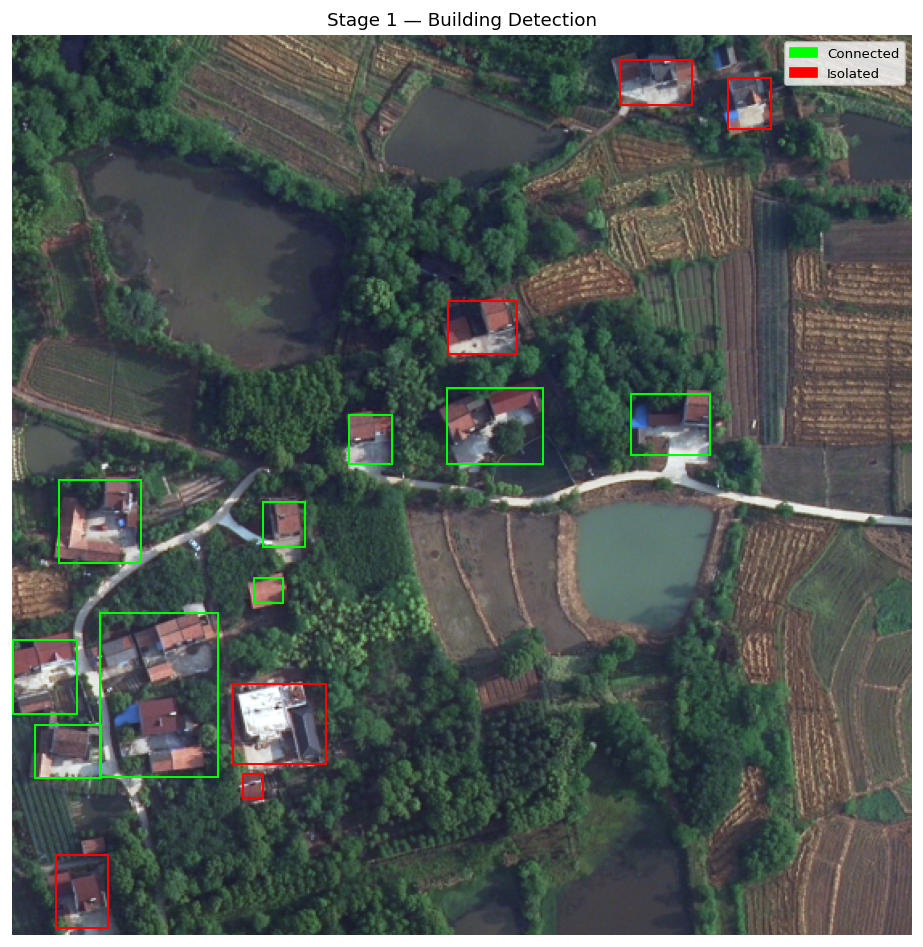
\includegraphics[width=0.48\textwidth]{figs/fig3_before.png}\hfill
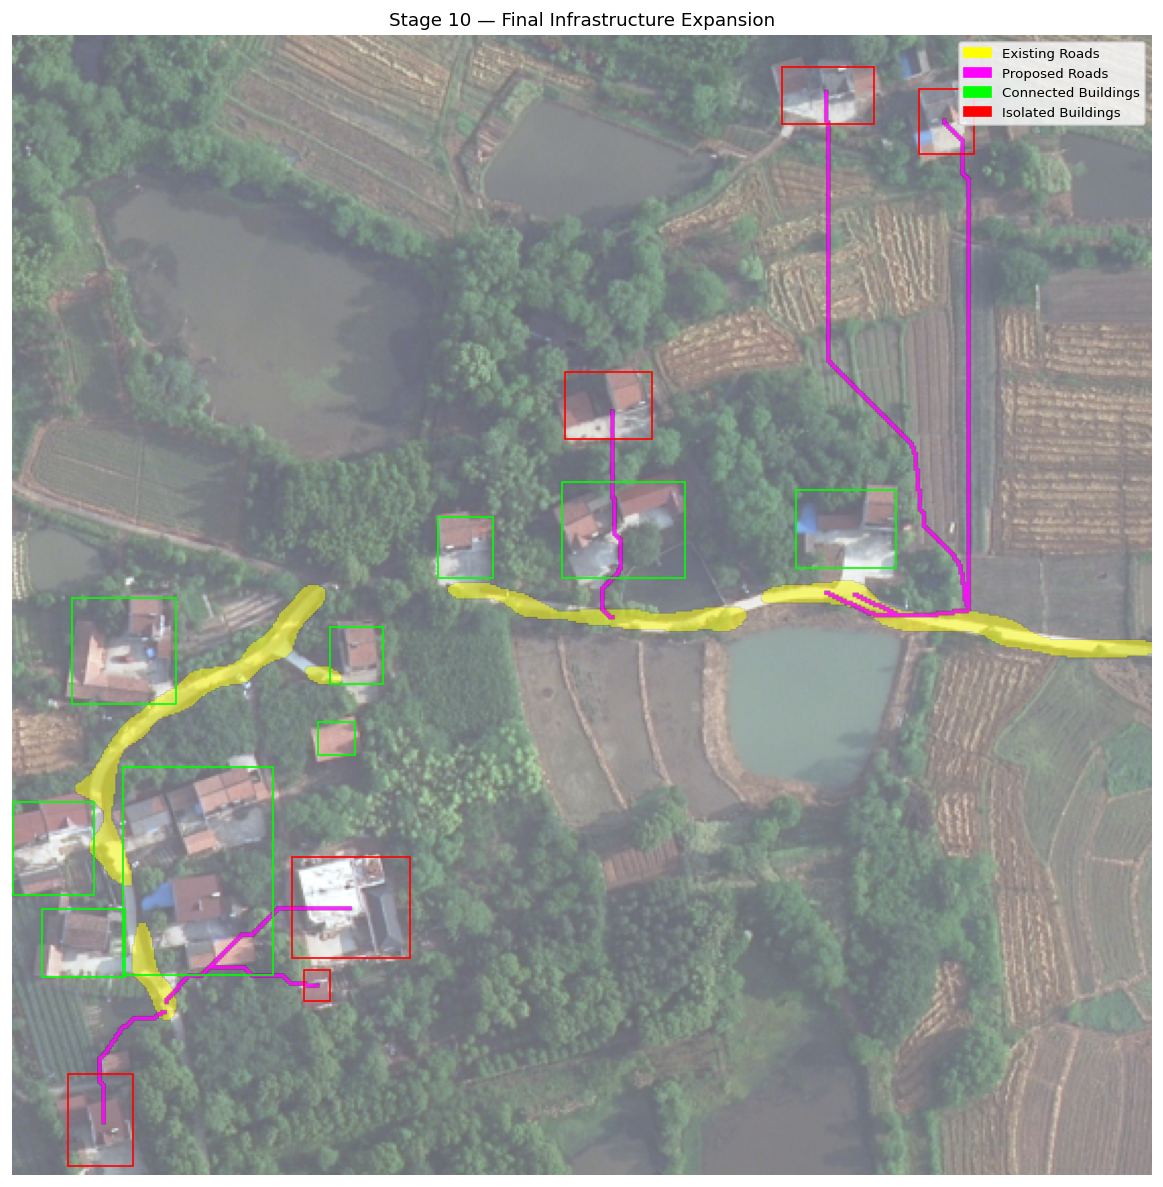
\includegraphics[width=0.48\textwidth]{figs/fig3_after.png}
\caption{Tile 4216 before (left) and after (right) planning. Green boxes: road-connected buildings (4); red: isolated (10); yellow: existing roads; magenta: A$^{*}$-planned connections.}\label{fig:plan}
\end{figure}

\subsection{Multi-Tile and Aggregate Evaluation}
On ten LoveDA rural tiles ($r=5$ px, 20 px min.\ area), tiles 4217/4225 had no detected buildings and tiles 4219/4222 stayed at 0\% (empty skeleton, no KD-tree target) -- so 100\% post-planning connectivity is not general. Table~\ref{tab:tile10} (right): 54 buildings, connectivity 40.74\%$\to$96.30\% (+55.56 points) via 30 connections, path efficiency $0.931\pm0.026$ over 8 path-feasible tiles. Tile 4216's composition (Background 15.9\%, Building 12.9\%, Road 1.4\%, Water 3.4\%, Forest 48.5\%, Agriculture 17.9\%) matched per-class pixel counts.

\subsection{Discussion}
Water scores highest on IoU/F1 (71.91\%/83.66\%), followed by Building (66.77\%/80.08\%), in line with lightweight segmenters such as UNetFormer~\cite{wang2022unet} (benchmarks differ, so no direct comparison). Background recall (80.57\%) exceeds precision (62.09\%, over-prediction); Agriculture shows the opposite (87.58\%/62.61\%, conservative); Barren and Forest remain weakest (30.13\%/39.86\% IoU); Road's 56.44\% IoU with 64.14\% recall makes broken road masks a realistic planner failure mode. Missed buildings and broken roads propagate into the component analysis, skeleton graph, and A$^{*}$ planning, so the 100\% post-planning connectivity is algorithmic, pixel-space connectivity on the selected tiles, not field-validated infrastructure -- matching GIS accessibility studies~\cite{verma2020,kapoor2021} where network quality and prioritisation, not raw counts, determine real gains. With an empty skeleton the KD-tree has no target, so proposed-road count, length, efficiency, and nearest-road distance become the more informative outputs.

%%ADD_BEGIN
\subsection{Additional Planning Scenes}\label{sec:scenes}
Table~\ref{tab:scenes} reports the planner ($r=5$ px) on two further scenes and a multi-tile batch. Tile 4208 (also the radius-sweep tile of Table~\ref{tab:tile10}, left) is moderately connected: 46.67\% $\to$ 100\% via 8 links. Tile 4200 is an isolated hamlet with a sparse road fragment: only 100 road pixels (0.0\%) were detected, so all 16 routes target that single fragment and are long (mean 413.49 px, about 227\,m). The multi-tile row covers the first 20 Rural validation tiles, retaining only tiles with at least one building and one proposed route (5 of 20; of the rest, 13 had no building and 2 had buildings but no plannable route). It is therefore the \emph{active-road plannable subset}, not an unbiased sample, and complements the ten-tile summary above.

\begin{table}[t]
\caption{Additional planning scenes ($r=5$ px). The multi-tile row is the active-road plannable subset (5 of the first 20 Rural validation tiles), per-tile means.}\label{tab:scenes}
\centering
\resizebox{\columnwidth}{!}{%
\begin{tabular}{lrrrrrr}
\toprule
Scene & Buildings & Conn.\ before $\to$ after (\%) & Links & Length (px) & Mean (px) & Eff.\\
\midrule
4208.png & 15 & 46.67 $\to$ 100.00 & 8 & 1,130.10 & 141.26 & 0.8502\\
4200.png & 16 & 0.00 $\to$ 100.00 & 16 & 6,615.88 & 413.49 & 0.9300\\
Multi-tile (active subset) & 8.20 & 6.67 $\to$ 100.00 & 7.60 & 1,627.81 & -- & 0.93\\
\bottomrule
\end{tabular}}
\end{table}

\subsection{Domain-Adapted Baseline Comparison}\label{sec:sota}
SegFormer-B2 and DeepLabV3-R101 were fine-tuned from their public pretrained weights on the 2,522-tile LoveDA training split at $560\times560$ (AdamW, lr $=1.5\times10^{-4}$, 3 epochs, cross-entropy ignoring index 0, mixed precision) and compared with StrongDINOv2Seg on a 100-tile Rural validation subset against the official pixel-level ground truth (classes 1--7; Tesla T4, batch size 1, after warm-up). The protocol uses \emph{equal LoveDA training data under a short fixed 3-epoch schedule}, not identical tuning budgets: StrongDINOv2Seg is the epoch-4 checkpoint selected on validation mIoU, which favours it, whereas the baselines may be under-trained. Table~\ref{tab:sota} scores the 100-tile subset; its 43.11\% mIoU must not be compared with the 53.80\% mIoU (68.91\% mDice) of Table~\ref{tab:seg}, which is on the full validation split.

\begin{table}[t]
\caption{Baselines fine-tuned on LoveDA, scored on the 100-tile Rural validation subset (not the full validation split of Table~\ref{tab:seg}); T4 GPU, $560\times560$, latency mean $\pm$ std.}\label{tab:sota}
\centering
\resizebox{\columnwidth}{!}{%
\begin{tabular}{lrrrrr}
\toprule
Model & mIoU (\%) & mDice (\%) & Building IoU (\%) & Road IoU (\%) & Latency (ms)\\
\midrule
DeepLabV3-R101 (LoveDA) & 32.38 & 47.41 & 33.50 & 28.80 & $176.36\pm2.98$\\
SegFormer-B2 (LoveDA) & 37.22 & 50.95 & 32.49 & \textbf{34.90} & $\mathbf{64.19}\pm3.23$\\
StrongDINOv2Seg (ours) & \textbf{43.11} & \textbf{56.62} & \textbf{62.40} & 34.79 & $145.34\pm1.75$\\
\bottomrule
\end{tabular}}
\end{table}

StrongDINOv2Seg gains $+5.89$ mIoU over SegFormer-B2 and $+10.73$ over DeepLabV3-R101, driven by Building IoU ($+29.91$ over SegFormer-B2). Road IoU is on par with SegFormer-B2 (34.79\% vs.\ 34.90\%), so no road advantage is claimed, and SegFormer-B2 is about $2.3\times$ faster (64.19 vs.\ 145.34\,ms). The low Road IoU of all models reflects thin, partly canopy-occluded rural tracks, which the skeletonization and A$^{*}$ stages tolerate by linking each isolated building to the nearest detected road pixel; where no road is detected the planner has no target (Sect.~\ref{sec:scenes}).
%%ADD_END

\section{Limitations and Future Work}
\textbf{Evaluation split.} All segmentation numbers come from the LoveDA validation split, which also guided epoch selection, so no held-out test set was used and results carry model-selection bias. %%LIM_OLD
No local baselines or ablation. Figures for other methods (Sect.~\ref{sec:r2}) come from their papers rather than identical retraining here, and isolating the FPN, ASPP, and decoder's individual contributions is left for future work; this is a demonstration, not proof of outperforming any baseline. %%LIM_END
\textbf{Planning scope and failure modes.} Results cover only the ten selected LoveDA tiles (Table~\ref{tab:tile10}); 100\% connectivity is not a general guarantee and fails outright where no road pixels are detected (tiles 4219, 4222), and no proposed route has been checked for engineering, legal, terrain, environmental, cost, or social feasibility -- the Bresenham fallback can cross impassable terrain. \textbf{Heuristic costs and units.} A$^{*}$ costs are heuristic, not calibrated construction costs, and distances remain in pixels rather than the georeferenced units OSMnx~\cite{boeing2017} could provide. \textbf{Generalisation.} Ten tiles is a small sample for judging generalisation; segmentation errors propagate downstream, and Rural/Urban LoveDA domains were trained jointly without separate evaluation.

\section{Conclusion}
StrongDINOv2Seg integrates DINOv2-based segmentation, graph-based connectivity analysis, and cost-weighted A$^{*}$ planning for rural infrastructure decision support, reaching a best validation mIoU of 53.80\% and mDice of 68.91\% on Rural/Urban LoveDA. Connectivity rose from 28.57\% to 100\% on the representative tile (10 connections, efficiency 0.86) and from 40.74\% to 96.30\% over ten tiles (30 connections, efficiency $0.931\pm0.026$). The contribution is the integrated pipeline, not any single component, and outputs are raster-based connectivity proposals, not field-validated or construction-ready plans; baseline reproduction, expert validation, georeferenced planning, and broader evaluation with GIS prioritisation frameworks~\cite{verma2020,kapoor2021} are future work.

\begin{credits}
\subsubsection{\discintname}
The authors declare that they have no known competing financial interests or personal relationships that could have appeared to influence the work reported in this paper.
\end{credits}

